%%%%%%%%%%%%%%%%%%%%%%%%%%%%%%%%%%%%%%%%%
% Beamer Presentation
% LaTeX Template
% Version 2.0 (March 8, 2022)
%
% This template originates from:
% https://www.LaTeXTemplates.com
%
% Author:
% Vel (vel@latextemplates.com)
%
% License:
% CC BY-NC-SA 4.0 (https://creativecommons.org/licenses/by-nc-sa/4.0/)
%
%%%%%%%%%%%%%%%%%%%%%%%%%%%%%%%%%%%%%%%%%

%----------------------------------------------------------------------------------------
%	PACKAGES AND OTHER DOCUMENT CONFIGURATIONS
%----------------------------------------------------------------------------------------
\documentclass[
	12pt, % Set the default font size, options include: 8pt, 9pt, 10pt, 11pt, 12pt, 14pt, 17pt, 20pt
	%t, % Uncomment to vertically align all slide content to the top of the slide, rather than the default centered
	aspectratio=169, % Uncomment to set the aspect ratio to a 16:9 ratio which matches the aspect ratio of 1080p and 4K screens and projectors
]{beamer}

\graphicspath{{Images/}{./}} % Specifies where to look for included images (trailing slash required)

\usepackage{booktabs} % Allows the use of \toprule, \midrule and \bottomrule for better rules in tables

%----------------------------------------------------------------------------------------
%	SELECT LAYOUT THEME
%----------------------------------------------------------------------------------------

% Beamer comes with a number of default layout themes which change the colors and layouts of slides. Below is a list of all themes available, uncomment each in turn to see what they look like.

%\usetheme{default}
%\usetheme{AnnArbor}
%\usetheme{Antibes}
%\usetheme{Bergen}
%\usetheme{Berkeley}
%\usetheme{Berlin}
\usetheme{Boadilla} %me gusta
%\usetheme{CambridgeUS}
%\usetheme{Copenhagen}
%\usetheme{Darmstadt}
%\usetheme{Dresden}
%\usetheme{Frankfurt}
%\usetheme{Goettingen} %dos dos
%\usetheme{Hannover} %dos dos
%\usetheme{Ilmenau}
%\usetheme{JuanLesPins}
%\usetheme{Luebeck}
%\usetheme{Madrid}
%\usetheme{Malmoe}
%\usetheme{Marburg}
%\usetheme{Montpellier}
%\usetheme{PaloAlto}
%\usetheme{Pittsburgh}
%\usetheme{Rochester} %muy flat
%\usetheme{Singapore}
%\usetheme{Szeged}
%\usetheme{Warsaw}

%----------------------------------------------------------------------------------------
%	SELECT COLOR THEME
%----------------------------------------------------------------------------------------

% Beamer comes with a number of color themes that can be applied to any layout theme to change its colors. Uncomment each of these in turn to see how they change the colors of your selected layout theme.

%\usecolortheme{albatross}
%\usecolortheme{beaver}
%\usecolortheme{beetle}
%\usecolortheme{crane}
%\usecolortheme{dolphin}
%\usecolortheme{dove}
%\usecolortheme{fly}
%\usecolortheme{lily} %default
%\usecolortheme{monarca}
%\usecolortheme{seagull}
%\usecolortheme{seahorse}
%\usecolortheme{spruce}
%\usecolortheme{whale}
%\usecolortheme{wolverine}

%----------------------------------------------------------------------------------------
%	SELECT FONT THEME & FONTS
%----------------------------------------------------------------------------------------

% Beamer comes with several font themes to easily change the fonts used in various parts of the presentation. Review the comments beside each one to decide if you would like to use it. Note that additional options can be specified for several of these font themes, consult the beamer documentation for more information.

\usefonttheme{default} % Typeset using the default sans serif font
%\usefonttheme{serif} % Typeset using the default serif font (make sure a sans font isn't being set as the default font if you use this option!)
%\usefonttheme{structurebold} % Typeset important structure text (titles, headlines, footlines, sidebar, etc) in bold
%\usefonttheme{structureitalicserif} % Typeset important structure text (titles, headlines, footlines, sidebar, etc) in italic serif
%\usefonttheme{structuresmallcapsserif} % Typeset important structure text (titles, headlines, footlines, sidebar, etc) in small caps serif

%------------------------------------------------

%\usepackage{mathptmx} % Use the Times font for serif text
\usepackage{palatino} % Use the Palatino font for serif text

\usepackage[ruled,vlined]{algorithm2e}
%\usepackage{helvet} % Use the Helvetica font for sans serif text
\usepackage[default]{opensans} % Use the Open Sans font for sans serif text
\usepackage[spanish]{babel}
\usepackage{dirtree}
\usepackage{xcolor}
%\usepackage[default]{FiraSans} % Use the Fira Sans font for sans serif text
%\usepackage[default]{lato} % Use the Lato font for sans serif text

\usepackage[scaled]{helvet}
\usepackage[round]{natbib}
%\newcommand{\newblock}{}

\usepackage{rotating}

\newcommand\FourQuad[4]{%
  \begin{minipage}[b][.33\textheight][t] 
    {.48\textwidth}#1\end{minipage}\hfill%
    \begin{minipage}[b][.33\textheight][t] 
      {.48\textwidth}#2\end{minipage}\\[0.5em]
      \begin{minipage}[b][.33\textheight][t] 
        {.48\textwidth}#3\end{minipage}\hfill
        \begin{minipage}[b][.33\textheight][t] 
          {.48\textwidth}#4\end{minipage}%
}

\usepackage{tikz}
%\usetikzlibrary{arrows,shapes,positioning,shadows,trees,quotes}


%\tikzset{
%  basic/.style  = {draw, text width=2cm, drop shadow, font=\sffamily, rectangle},
%  root/.style   = {basic, rounded corners=2pt, thin, align=center,
%                   fill=green!30},
%  level 2/.style = {basic, rounded corners=6pt, thin,align=center, fill=green!60,
%                   text width=8em},
%  level 3/.style = {basic, thin, align=left, fill=pink!60, text width=6.5em}
%}

\usetikzlibrary{calc}

\tikzstyle{part} = [rectangle, rounded corners, minimum width=3cm, minimum height=1cm,     align=center, draw=black]
\tikzstyle{chapter} = [rectangle, rounded corners, minimum width=3cm, minimum height=1cm,     align=center, draw=black, text width=3.5cm]
\tikzstyle{arrow} = [thick, ->]

\usepackage{array} % needed for \arraybackslash
\usepackage{graphicx}
\usepackage{adjustbox} % for \adjincludegraphics

\usepackage{subcaption}
\usepackage{bibentry}
%\bibliographystyle{apalike}
\usepackage{chngcntr}
\usepackage{lipsum}% http://ctan.org/pkg/lipsum
\usepackage{hanging}% http://ctan.org/pkg/hanging

\usepackage{xcolor,colortbl}
\usepackage{multirow}

\usepackage{animate}
\usepackage{multicol}
\usepackage{tabularx,booktabs}
\usepackage{forloop}
\usepackage{ragged2e}

\usepackage{bbding} %palomitas checkmark
\usepackage{pifont}

\newcounter{loopcntr}
%----------------------------------------------------------------------------------------
%	SELECT INNER THEME
%----------------------------------------------------------------------------------------

% Inner themes change the styling of internal slide elements, for example: bullet points, blocks, bibliography entries, title pages, theorems, etc. Uncomment each theme in turn to see what changes it makes to your presentation.

%\useinnertheme{default}
\useinnertheme{circles}
%\useinnertheme{rectangles}
%\useinnertheme{rounded}
%\useinnertheme{inmargin}

%----------------------------------------------------------------------------------------
%	SELECT OUTER THEME
%----------------------------------------------------------------------------------------

% Outer themes change the overall layout of slides, such as: header and footer lines, sidebars and slide titles. Uncomment each theme in turn to see what changes it makes to your presentation.

%\useoutertheme{default}
%\useoutertheme{infolines}
%\useoutertheme{miniframes}
%\useoutertheme{smoothbars}
%\useoutertheme{sidebar}
%\useoutertheme{split}
%\useoutertheme{shadow}
%\useoutertheme{tree}
%\useoutertheme{smoothtree}

%\setbeamertemplate{footline} % Uncomment this line to remove the footer line in all slides
\setbeamertemplate{footline}[page number] % Uncomment this line to replace the footer line in all slides with a simple slide count
%\setbeamertemplate{caption}[numbered]
\setbeamertemplate{navigation symbols}{} % Uncomment this line to remove the navigation symbols from the bottom of all slides

%----------------------------------------------------------------------------------------
%	PRESENTATION INFORMATION
%----------------------------------------------------------------------------------------

\title[PROTOCOLO DE INVESTIGACIÓN]{%\centering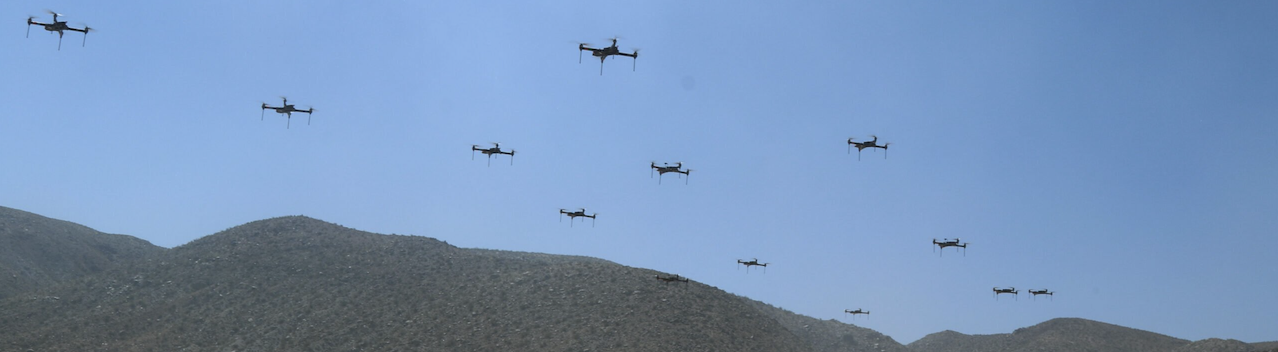
\includegraphics[width=10cm]{swarm_drones}\\
  Estrategias para la exploración coordinada multi-VANT} % The short title in the optional parameter appears at the bottom of every slide, the full title in the main parameter is only on the title page

%\subtitle{Optional Subtitle} % Presentation subtitle, remove this command if a subtitle isn't required

\author[Luis Ballado]{Luis Alberto Ballado Aradias} % Presenter name(s), the optional parameter can contain a shortened version to appear on the bottom of every slide, while the main parameter will appear on the title slide

\institute[CINVESTAV]{
  CINVESTAV UNIDAD TAMAULIPAS \\
  %\smallskip \textit{luis.ballado@cinvestav.mx}
} % Your institution, the optional parameter can be used for the institution shorthand and will appear on the bottom of every slide after author names, while the required parameter is used on the title slide and can include your email address or additional information on separate lines

\date[\today]{Cd. Victoria, Tamaulipas - \today} % Presentation date or conference/meeting name, the optional parameter can contain a shortened version to appear on the bottom of every slide, while the required parameter value is output to the title slide

%\titlegraphic{\hspace*{8.75cm}~%
%   
\includegraphics[width=0.8cm]{cinvestavlogo}
%}

%----------------------------------------------------------------------------------------

\counterwithin*{footnote}{page}
\newcommand\footcite[1]{\footnote{\bibentry{#1}}\label{\thepage:#1}}
\newcommand\secondcite[1]{\textsuperscript{\ref{\thepage:#1}}}

\newcommand{\rpt}[2][1]{%
  \forloop{loopcntr}{0}{\value{loopcntr}<#1}{#2}%
}
\newcommand{\on}[1][1]{
  \forloop{loopcntr}{0}{\value{loopcntr}<#1}{&\cellcolor{gray}}
}
\newcommand{\off}[1][1]{
  \forloop{loopcntr}{0}{\value{loopcntr}<#1}{&}
}

\addtolength{\textheight}{90pt}

\newcommand{\I}{\mathbb{I}}
\newcommand{\K}{\mathbb{K}}
\newcommand{\N}{\mathbb{N}}
\newcommand{\Q}{\mathbb{Q}}
\newcommand{\R}{\mathbb{R}}
\newcommand{\Z}{\mathbb{Z}}

\newcommand{\specialcell}[2][c]{%
  \begin{tabular}[#1]{@{}c@{}}#2\end{tabular}}


\begin{document}

%----------------------------------------------------------------------------------------
%	TITLE SLIDE
%----------------------------------------------------------------------------------------

\begin{frame}
  \titlepage % Output the title slide, automatically created using the text entered in the PRESENTATION INFORMATION block above
\end{frame}

%----------------------------------------------------------------------------------------
%	TABLE OF CONTENTS SLIDE
%----------------------------------------------------------------------------------------

% The table of contents outputs the sections and subsections that appear in your presentation, specified with the standard \section and \subsection commands. You may either display all sections and subsections on one slide with \tableofcontents, or display each section at a time on subsequent slides with \tableofcontents[pausesections]. The latter is useful if you want to step through each section and mention what you will discuss.
\AtBeginSection[]
{
  \begin{frame}
    \frametitle{Contenido} % Slide title, remove this command for no title
    \tableofcontents[currentsection] % Output the table of contents (all sections on one slide)
    %\tableofcontents[pausesections] % Output the table of contents (break sections up across separate slides)
  \end{frame}
}
%----------------------------------------------------------------------------------------
%	PRESENTATION BODY SLIDES
%----------------------------------------------------------------------------------------

\section{Resumen}
\begin{frame}{Resumen}%{Problemática}
  \bigskip % Vertical whitespace
  \centering
  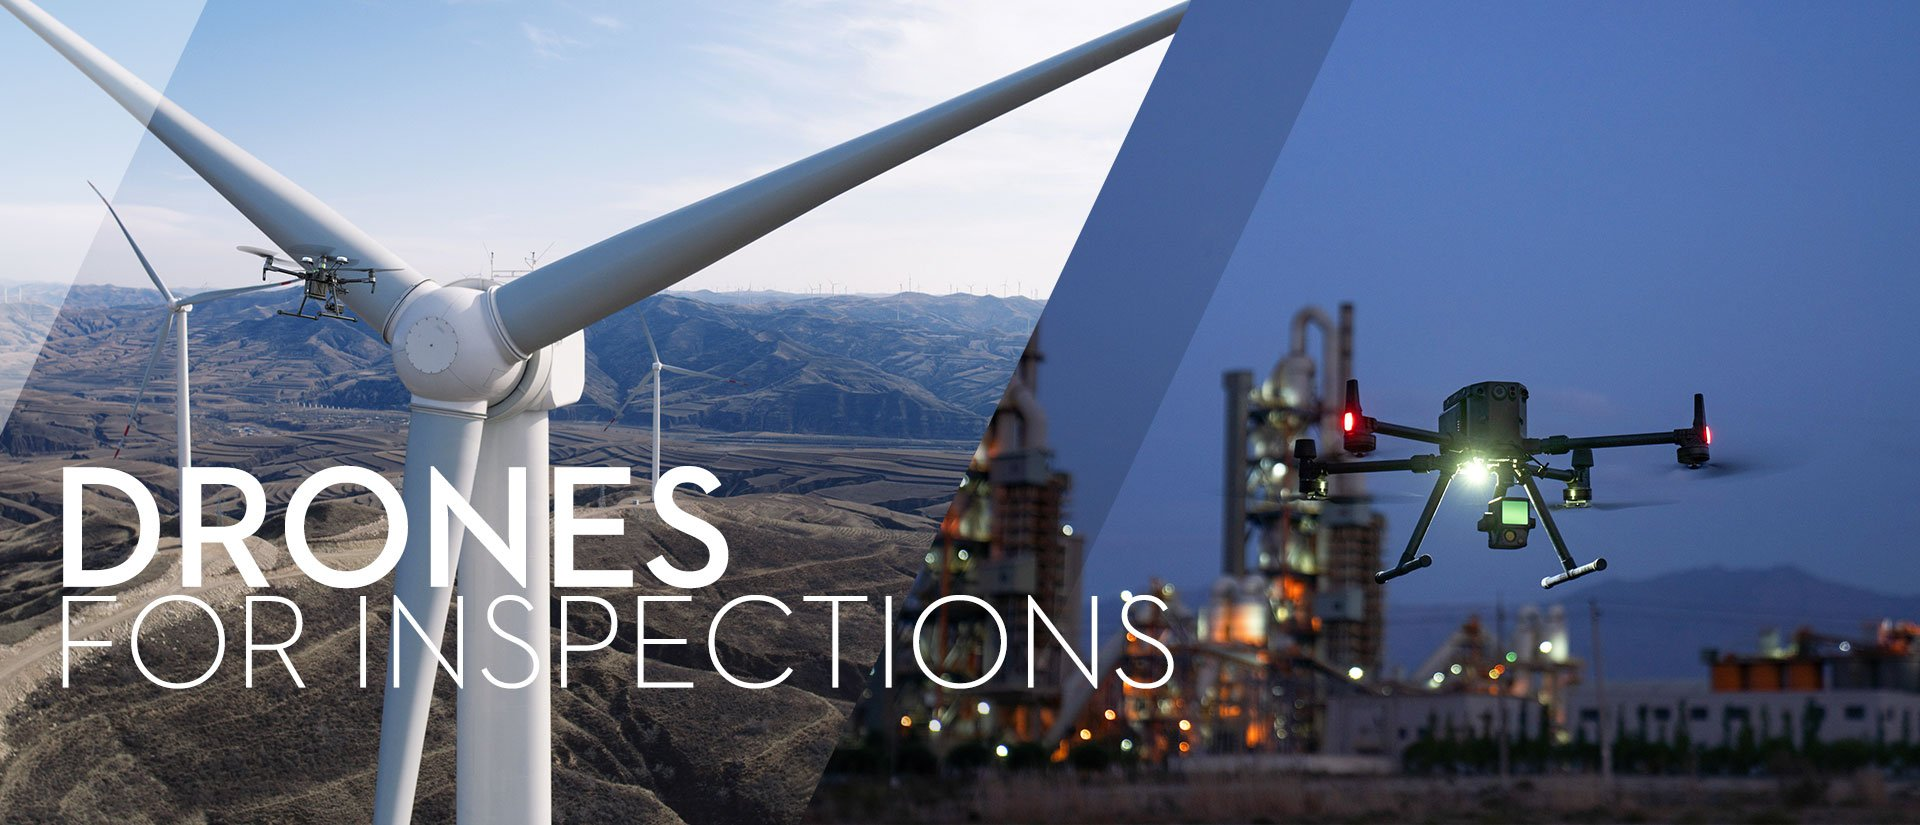
\includegraphics[width=0.45\textwidth,height=0.35\textheight]{DJI_B1}$^\dag$
  \hfil
  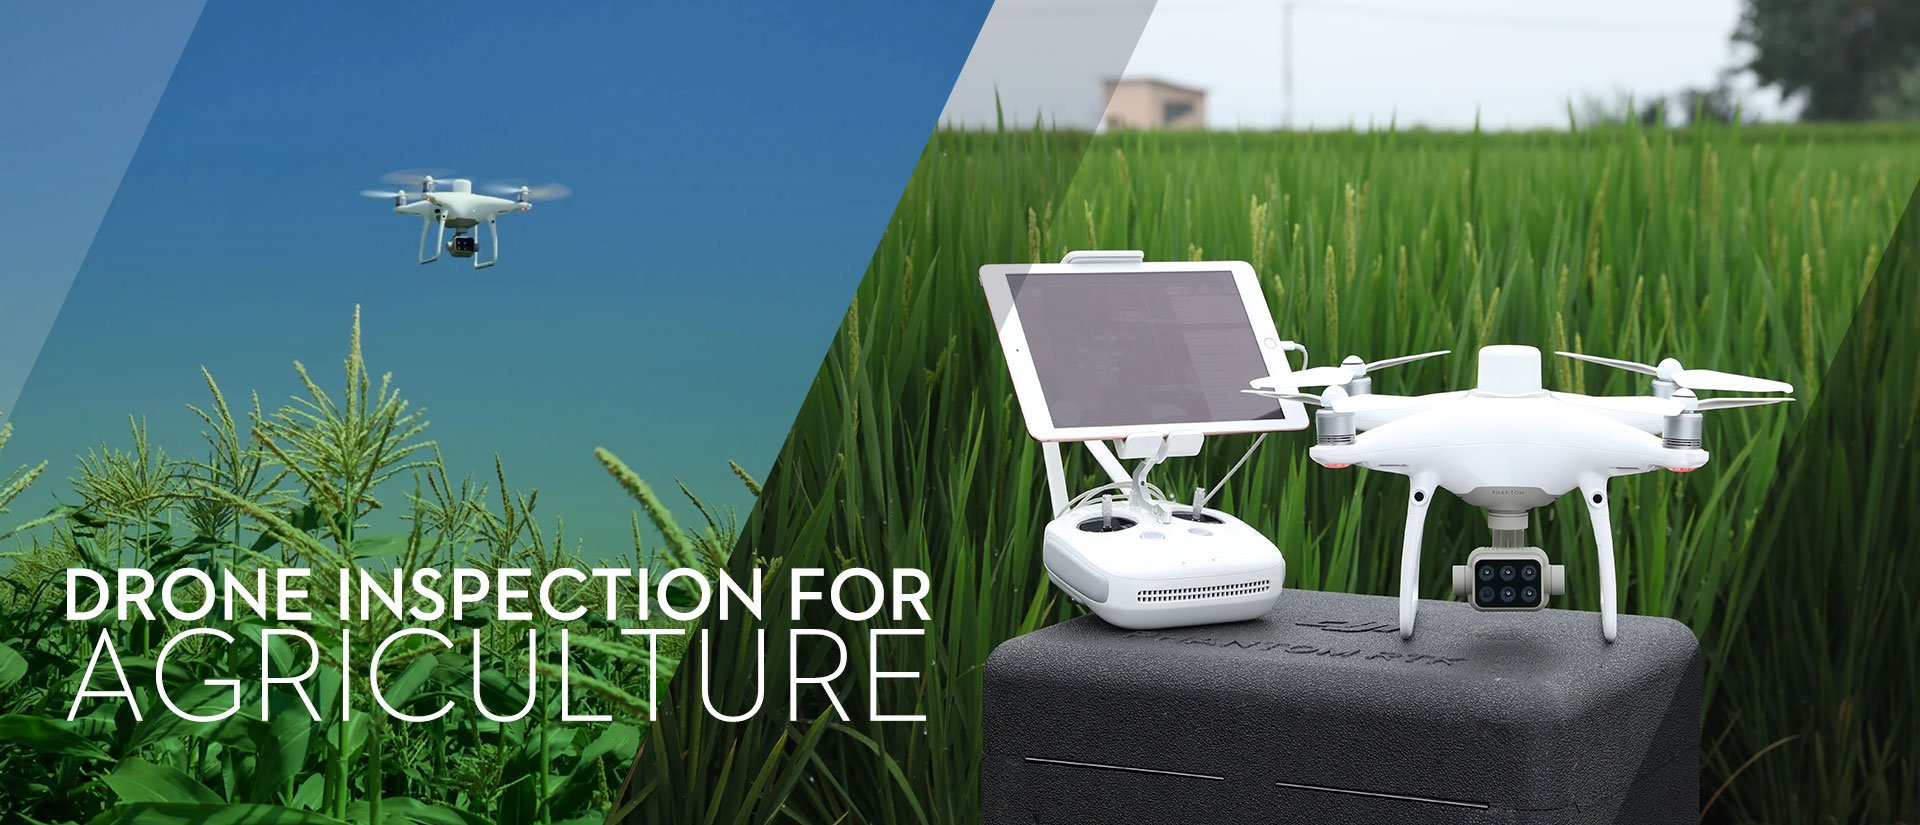
\includegraphics[width=0.45\textwidth,height=0.35\textheight]{DJI_B2}$^\dag$
  \vspace{2pt}
  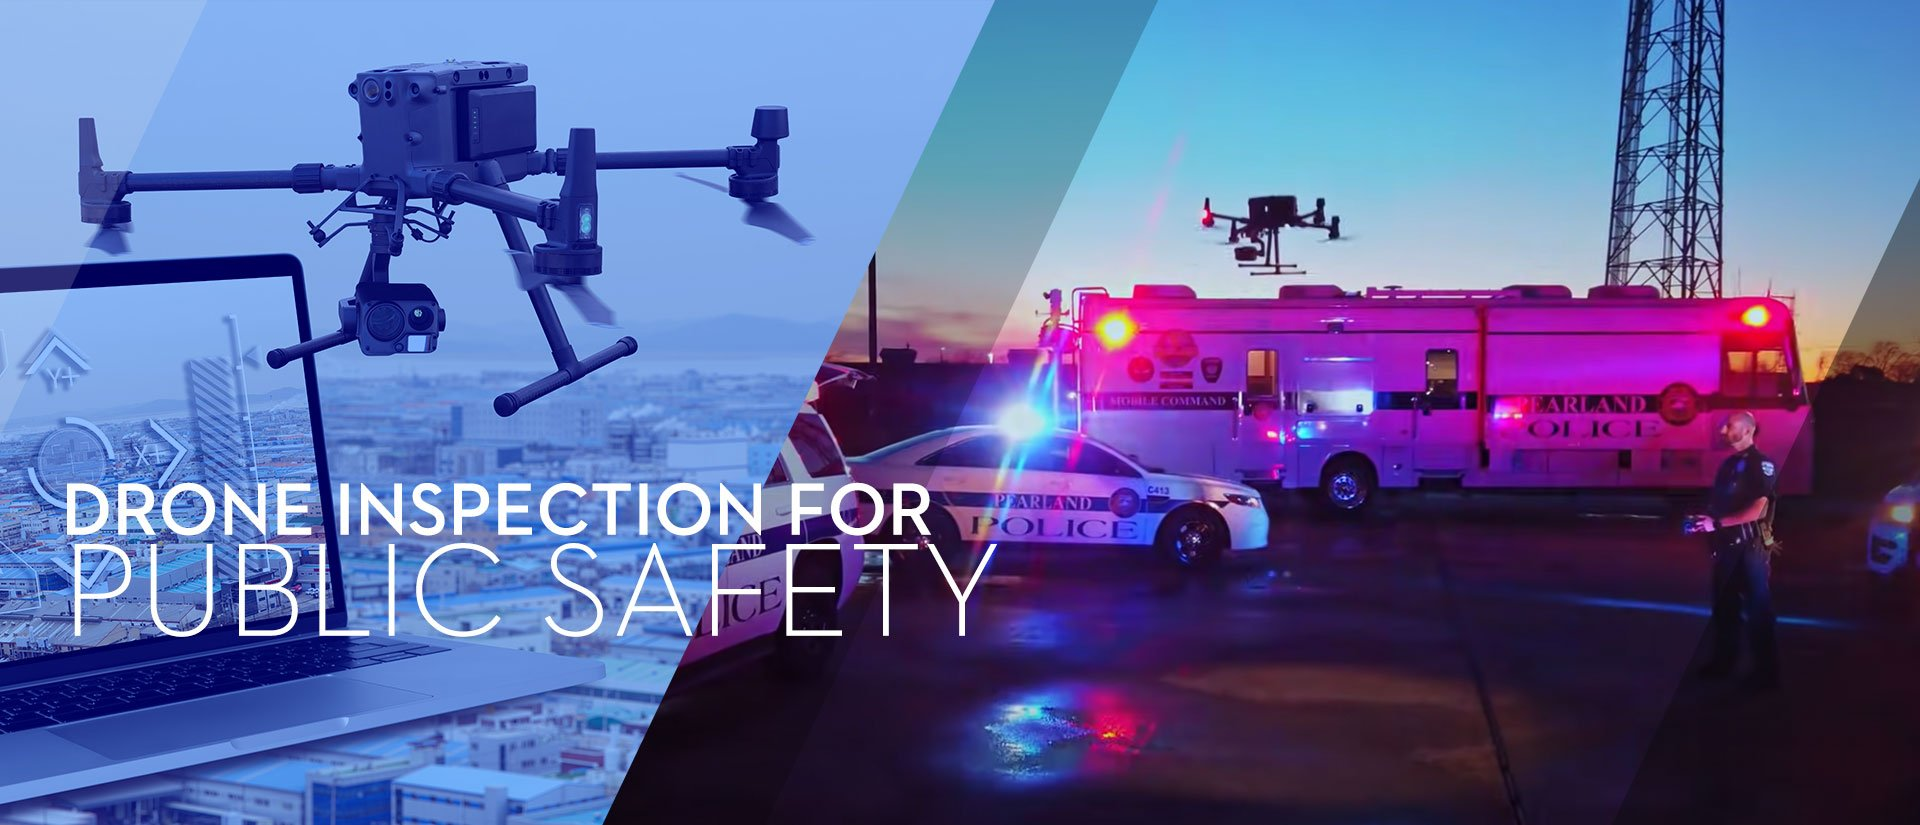
\includegraphics[width=0.45\textwidth,height=0.35\textheight]{DJI_B5}$^\dag$ 
  \hfil
  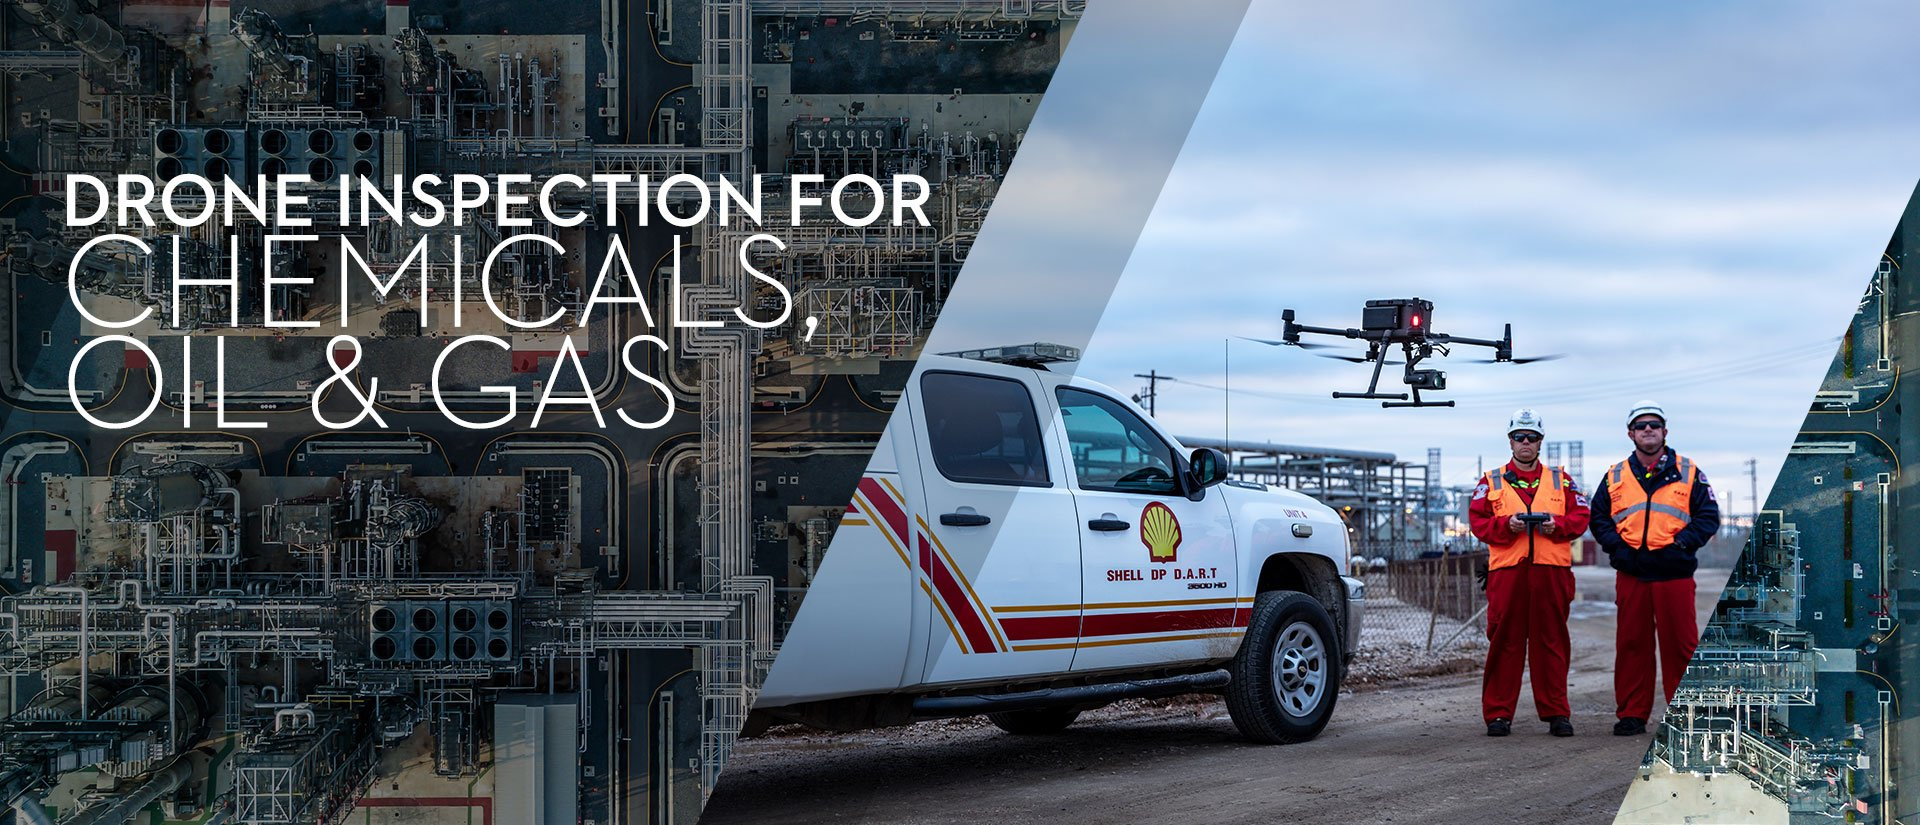
\includegraphics[width=0.45\textwidth,height=0.35\textheight]{DJI_B4}$^\dag$\\
  \rule{0in}{1.2em}$^\dag$ \small Drone Inspections Based on Best Use Cases \\
  \tiny \url{https://enterprise-insights.dji.com/blog/complete-guide-to-drone-inspections}
\end{frame}

\section{Descripción del proyecto}
\begin{frame}{Descripción del proyecto}
  \begin{minipage}{0.47\textwidth}
    \begin{itemize}
    \item<1-> Coordinación eficiente para la exploración multi-VANT 
    \item<2-> Optimizar la cobertura en entornos complejos
    \item<3-> Toma de decisiones colaborativa y asignación de tareas
    \item<4-> Evasión de obstáculos y coordinación en tiempo real
    \item<5-> Fusión de información (sensores y navegación)
    \end{itemize}
  \end{minipage}
  \begin{minipage}{0.5\textwidth}
    \only<1>{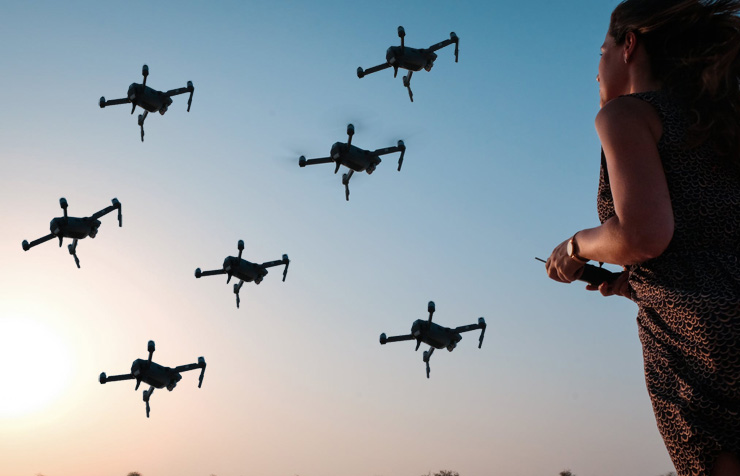
\includegraphics[width=\textwidth]{multiple-drones}$^\dag$\\
      \rule{0in}{1.2em}$^\dag$\scriptsize Hardware in the loop framework proposal for a semi-autonomous car architecture in a closed route environment \cite{CurielRamirez2019}
    }
    \only<2>{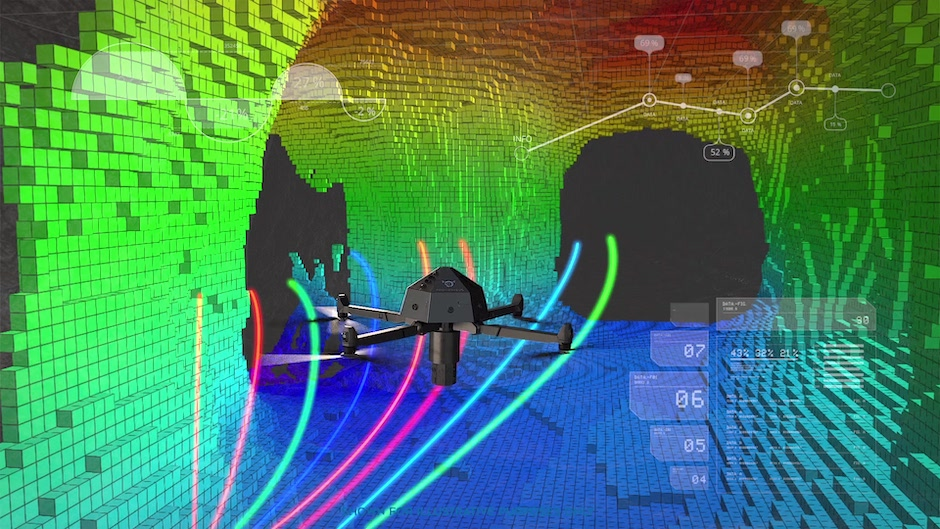
\includegraphics[width=\textwidth]{drone_path}$^\dag$\\
      \rule{0in}{1.2em}$^\dag$\scriptsize Hardware in the loop framework proposal for a semi-autonomous car architecture in a closed route environment \cite{CurielRamirez2019}
    }
    \only<3>{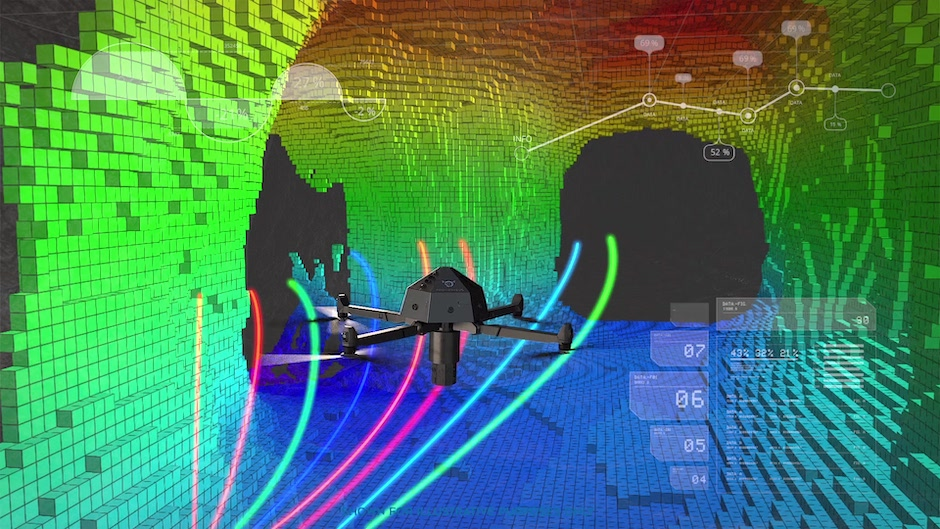
\includegraphics[width=\textwidth]{drone_path}$^\dag$\\
      \rule{0in}{1.2em}$^\dag$\scriptsize Hardware in the loop framework proposal for a semi-autonomous car architecture in a closed route environment \cite{CurielRamirez2019}
    }
    \only<4>{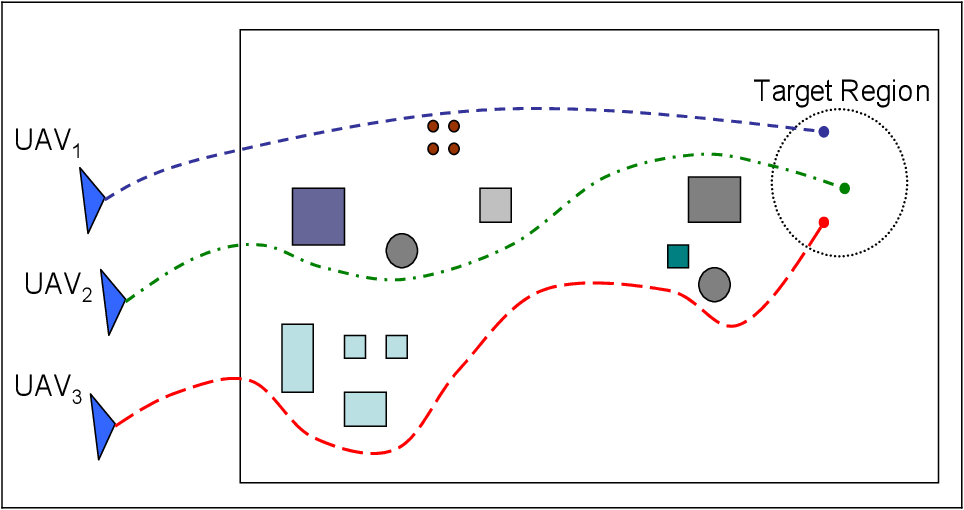
\includegraphics[width=\textwidth]{drone_collision}$^\dag$\\
      \rule{0in}{1.2em}$^\dag$\scriptsize Hardware in the loop framework proposal for a semi-autonomous car architecture in a closed route environment \cite{CurielRamirez2019}
    }
    \only<5>{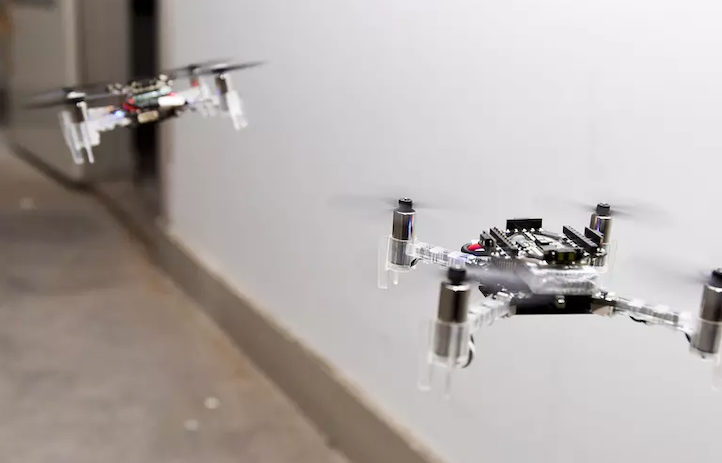
\includegraphics[width=\textwidth]{drone_action}$^\dag$\\
      \rule{0in}{1.2em}$^\dag$\scriptsize Hardware in the loop framework proposal for a semi-autonomous car architecture in a closed route environment \cite{CurielRamirez2019}
    }
  \end{minipage}
\end{frame}

\section{Antecedentes y motivación para el proyecto}
\begin{frame}{Arquitectura híbrida}
  \begin{figure}
    \centering
    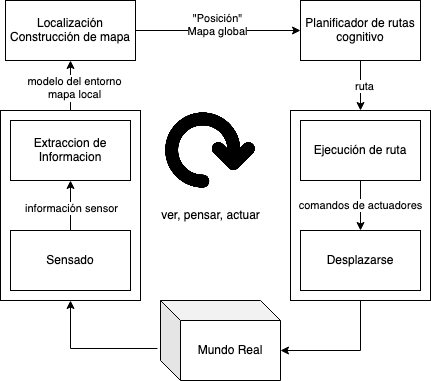
\includegraphics[scale=0.50]{sentir_pensar_actuar}$^\dag$\\
    \rule{0in}{1.2em}$^\dag$\scriptsize Hardware in the loop framework proposal for a semi-autonomous car architecture in a closed route environment \cite{CurielRamirez2019}\\
  \end{figure}
\end{frame}

\begin{frame}{Multi-robots}
  \begin{columns}
    \column{0.5\textwidth}
    Beneficios coordinación multi-VANT
    \begin{itemize}
    \item Eficiencia y cobertura
    \item Redundancia y tolerancia a fallos
    \item Adaptabilidad a entornos dinámicos
    \item Distribución de carga de trabajo
    \item Esfuerzo colaborativo
    \end{itemize}
    \column{0.5\textwidth}
    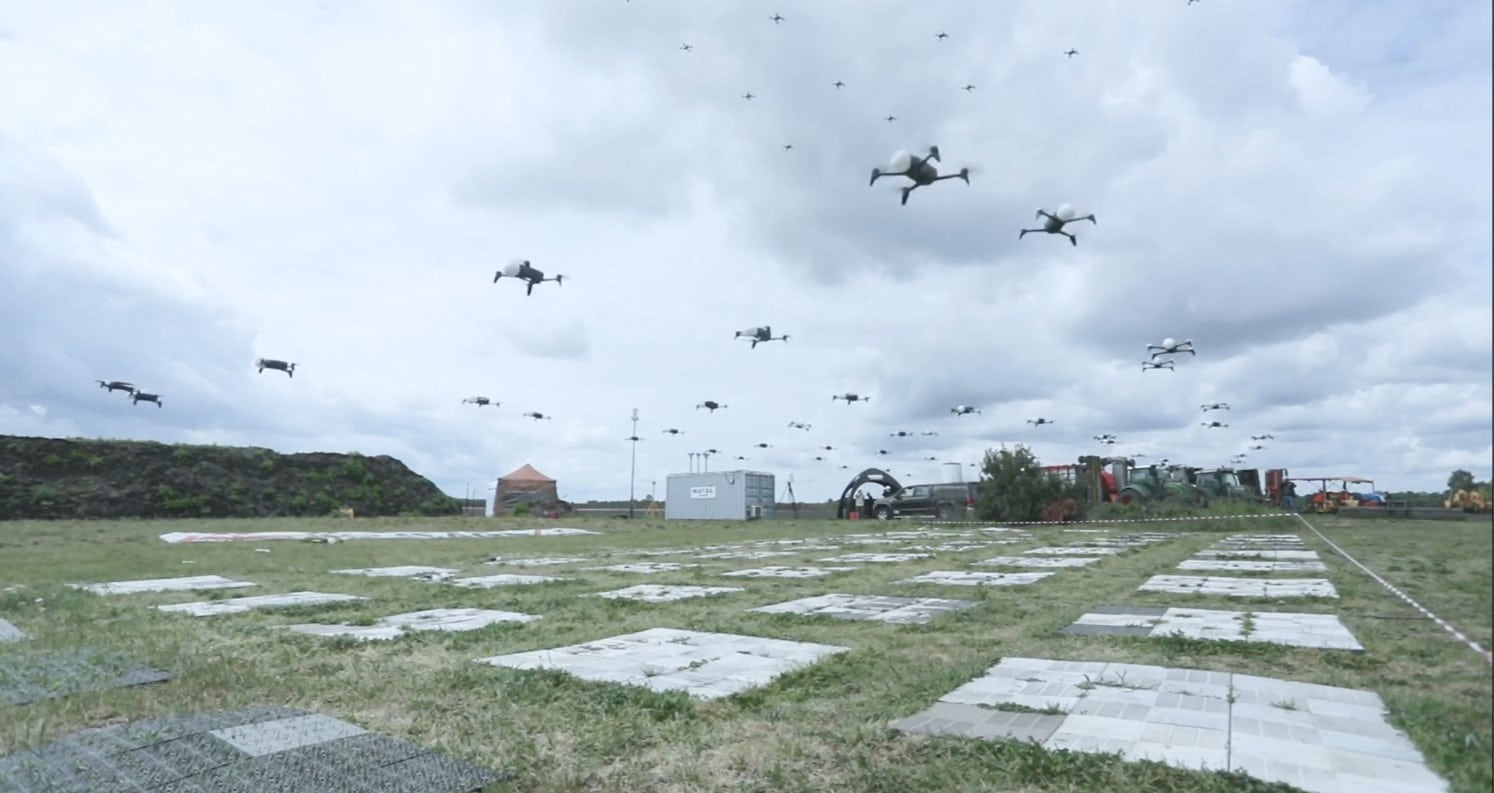
\includegraphics[width=\textwidth]{drone_swarm}$^\dag$\\
    \rule{0in}{1.2em}$^\dag$\scriptsize Hardware in the loop framework proposal for a semi-autonomous car architecture in a closed route environment \cite{CurielRamirez2019}
  \end{columns}
\end{frame}

\begin{frame}{Panorama Planificación de trayectorias}
  %\cite{nphard}[\citenum{nphard}] \cite{5427034}[\citenum{5427034}]
  %Calcular la ruta más corta entre dos puntos en un ambiente 3D es un problema NP-HARD.
  %La mayoria de planificadores de rutas hacen uso de heuristicas y metaheuristicas para
  %generar el óptimo más cercano \\
  \begin{figure}
    \centering
    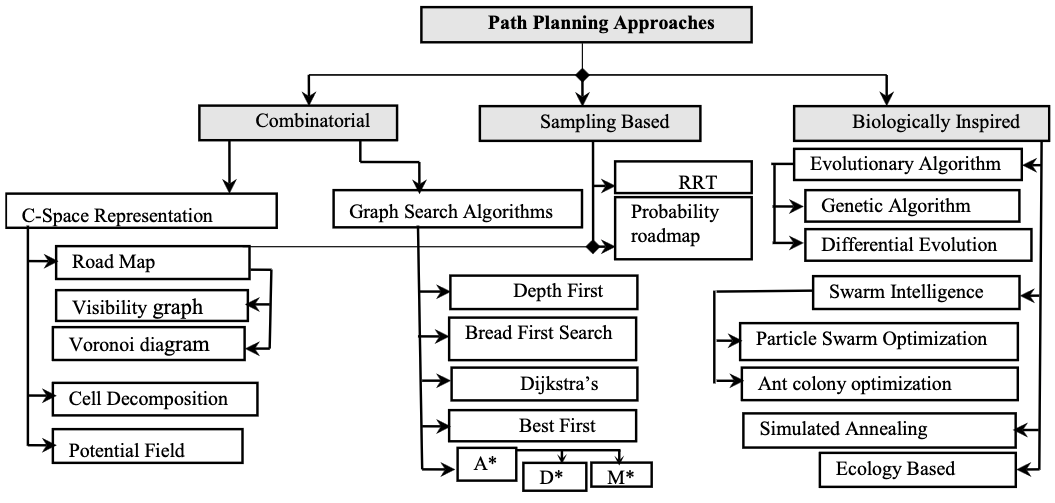
\includegraphics[scale=0.33]{path_planning_panorama}
    \caption[Caption for LOF]{Clasificación del enfoque de planificación de rutas\footnotemark}
  \end{figure}
  \footnotetext{Different Cell Decomposition Path Planning Methods for Unmanned Air Vehicles - A Review \cite{Debnath2020}}
\end{frame}

\begin{frame}{Representación del ambiente 3D}
  %MOSTRAR OCTOMAP
  %MOSTRAR MAPA 3D
  \begin{figure}
    \centering
    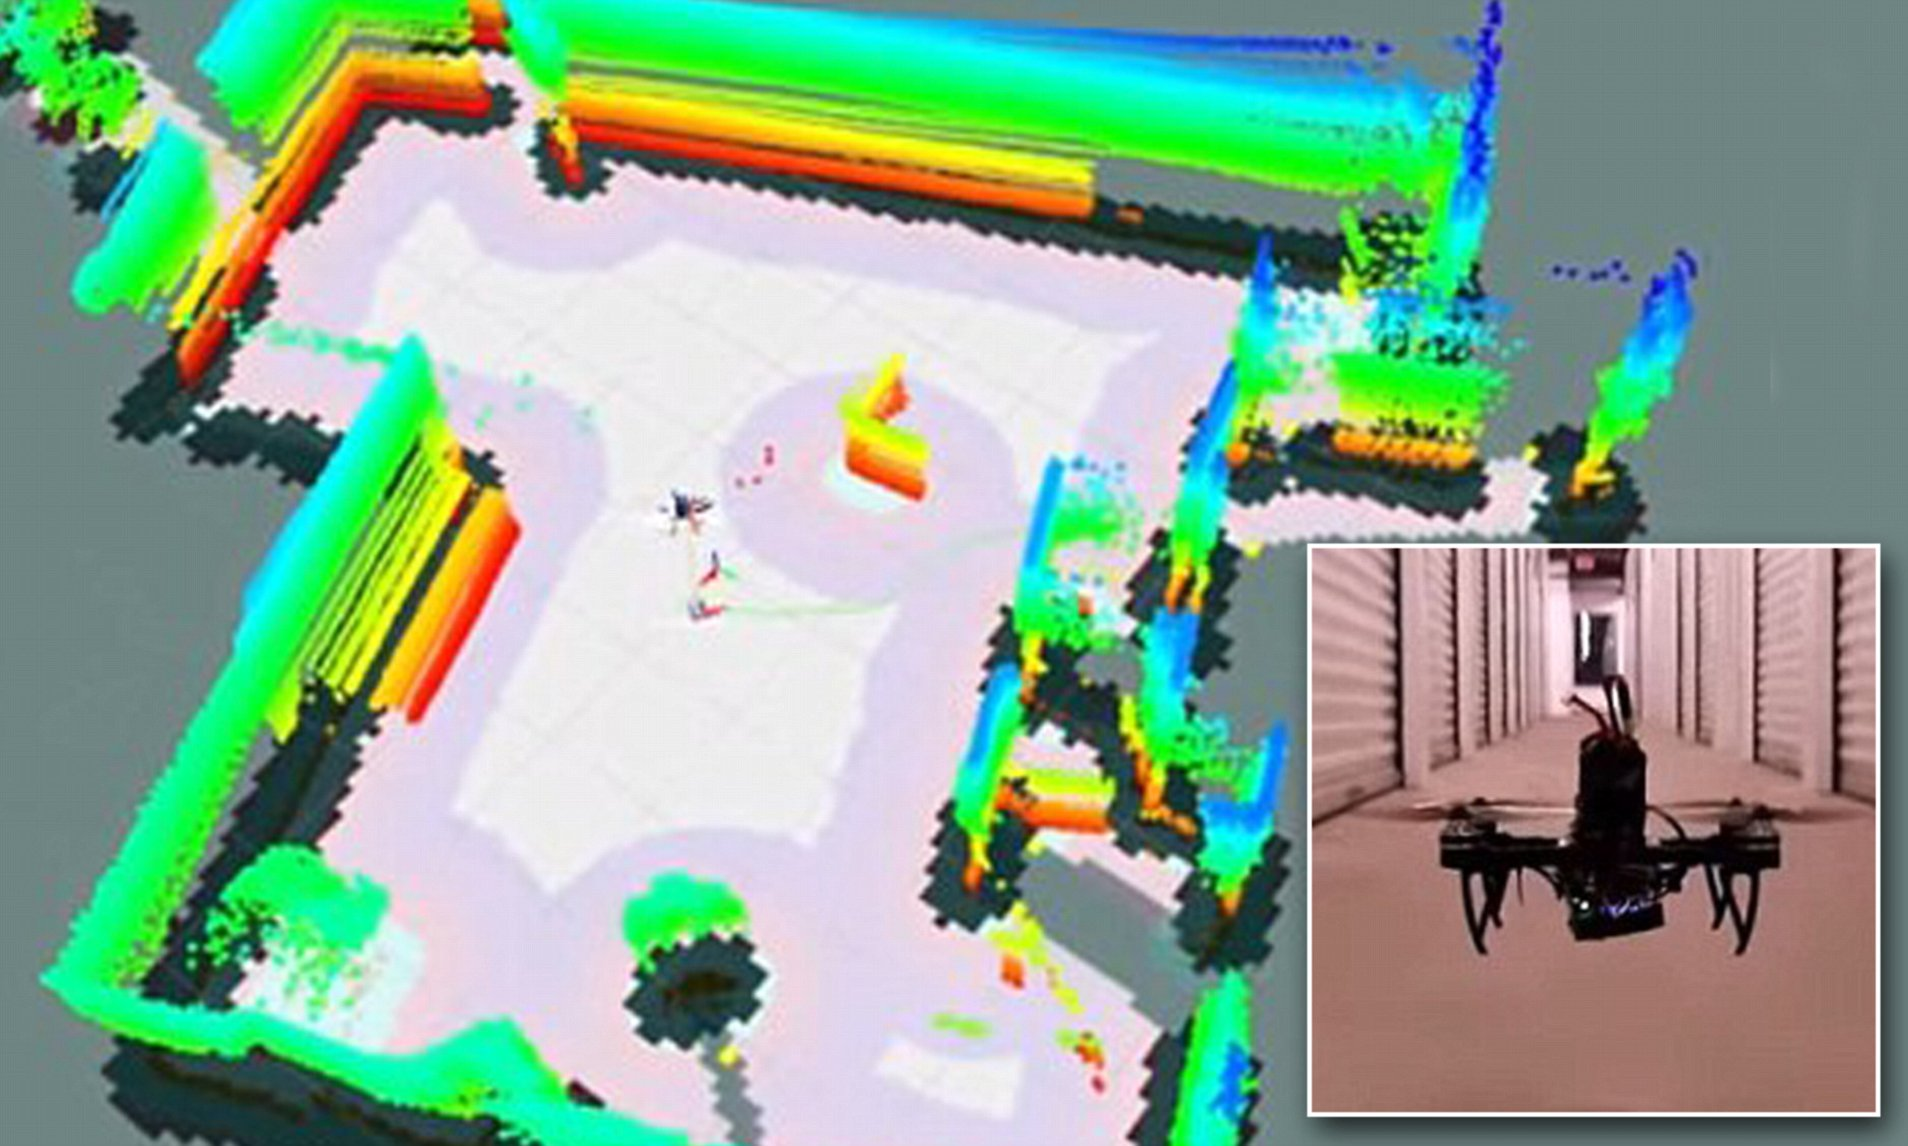
\includegraphics[scale=0.15]{drone_mapping}
    \caption[Caption for LOF]{Mapa probabilistico 3D\protect\footnotemark}
  \end{figure}
  \footnotetext{Cooperación en robots heterogeneos}
\end{frame}

\section{Planteamiento del problema}
\begin{frame}
  \frametitle{Planteamiento del problema}
  \begin{columns}
    \column{0.5\textwidth}
    \justifying
    \small Desarrollar una estrategia de exploración multi-VANT que reduzca el tiempo total de exploración dado un conjunto de $\mathcal{V}$ vehículos aéreos no tripulados. Las capacidades limitadas de energía y sensores abordo de los VANTS les permiten navegar de forma autónoma. Teniendo en cuenta sus limitaciones de energía y la necesidad de una exploración eficiente, el objetivo es determinar la trayectoria, las rutas y la asignación de tareas óptimas ó sub-óptimas.
    \column{0.5\textwidth}\\
    \pause
    \centering
    \small Retos multi-VANT
    \begin{itemize}
    \small \item Coordinación - Establecer comunicación efectiva entre los múltiples VANTs. Intercambiar información relevante. Tener baja latencia en su comunicación.
    \small \item Planificación - Los VANTs deben coordinar sus movimientos para evitar colisiones y lograr una cobertura eficiente del área objetivo.
    \small \item Asignación de tareas - Se busca evitar la duplicación de esfuerzos optimizando el uso de recursos disponibles.
    \end{itemize}
  \end{columns}
\end{frame}

\section{Objetivos generales y específicos del proyecto}
\begin{frame}
  \frametitle{Objetivos generales y específicos del proyecto}
  \begin{enumerate}
  \item<1-> General \\
    Diseñar una arquitectura de software descentralizada para implementar una estrategia multi-VANT capaz de resolver los problemas de localización y coordinación en ambientes desconocidos y dinámicos para tareas de exploración en interiores.
    \pause
  \item<2-> Particulares\\
    \begin{itemize}
    \item Diseño de solución en base a los algoritmos reportados en la literatura.
      \pause
    \item Valoración propuesta (simulación de propuesta).
      \pause
    \item Comparación y análisis (escalabilidad, robustez y recursos computacionales).
    \end{itemize}
  \end{enumerate}
\end{frame}

%Explicar con el cronograma
\section{Metodología}
\begin{frame}{Metodología/Cronograma}
  \begin{figure}
    \centering
    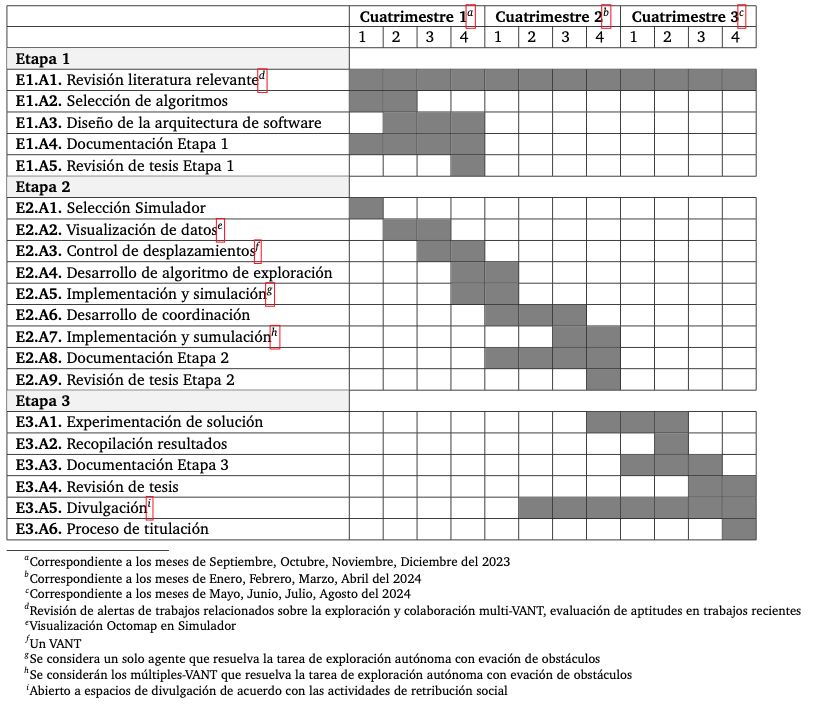
\includegraphics[width=11cm, height=8cm]{cronograma}
  \end{figure}
\end{frame}

\section{Estado del Arte}
\begin{frame}{Estado del Arte}
  \bigskip % Vertical whitespace
  \centering
  \begin{tabular}{ | p{4cm} | p{3cm} | p{2.5cm} | p{3.5cm}|}
    \hline
    \scriptsize REFERENCIA&
    \scriptsize REPRESENTACION&
    \scriptsize BUSQUEDA&
    \scriptsize Control de trayectoria\\
    \hline
    \hline
    %--------------------------
    \scriptsize \cite{CIESLEWSKI2017}[\citenum{CIESLEWSKI2017}]&
    \scriptsize Octomap&
    \scriptsize Basado en fronteras&
    \scriptsize Control directo de velocidad\\ \hline
    %--------------------------
    \scriptsize \cite{USENKO2017}[\citenum{USENKO2017}]&
    \scriptsize Cuadr\'{i}cula egoc\'{e}ntrica&
    \scriptsize Offline RRT*&
    \scriptsize Curvas de Bezier\\ \hline 
    %--------------------------
    \scriptsize \cite{MOHTA2017}[\citenum{MOHTA2017}]&
    \scriptsize mapa 3D-Local y 2D-Global&
    \scriptsize A*&
    \scriptsize Prograci\'{o}n cuadr\'{a}tica \\ \hline 
    %--------------------------
    \scriptsize \cite{LIN2017}[\citenum{LIN2017}]&
    \scriptsize 3D voxel array TSDF&
    \scriptsize A*&
    \scriptsize Optimizaci\'{o}n cuadr\'{a}tica \\ \hline
    %--------------------------
    \scriptsize \cite{PAPACHRISTOS2017}[\citenum{PAPACHRISTOS2017}]&
    \scriptsize Octomap&
    \scriptsize NBVP&
    \scriptsize Control directo de velocidad \\ \hline
    %--------------------------
    \scriptsize \cite{OLEYNIKOVA2018}[\citenum{OLEYNIKOVA2018}]&
    \scriptsize Voxel Hashing TSDF&
    \scriptsize NBVP&
    \scriptsize Optimizaci\'{o}n cuadr\'{a}tica \\ \hline
    %--------------------------
    \scriptsize \cite{GAO2018}[\citenum{GAO2018}]&
    \scriptsize Mapa de cuadr\'{i}cula&
    \scriptsize M\'{e}todo de marcha r\'{a}pida&
    \scriptsize Optimizaci\'{o}n cuadr\'{a}tica \\ \hline
  \end{tabular}
\end{frame}

\begin{frame}
  
  \centering
  \begin{tabular}{ | p{4cm} | p{3cm} | p{2.5cm} | p{3.5cm}|}
    \hline
    \scriptsize REFERENCIA&
    \scriptsize MAPA&
    \scriptsize Planificador de rutas&
    \scriptsize Control trayectoria\\
    \hline
    \hline
    %--------------------------
    \scriptsize \cite{FLORENCE2018}[\citenum{FLORENCE2018}]&
    \scriptsize Busqueda basada en visibilidad&
    \scriptsize 2D A*&
    \scriptsize Control MPC \\ \hline
    %--------------------------
    \scriptsize \cite{SELIN2019}[\citenum{SELIN2019}]&
    \scriptsize Octomap&
    \scriptsize NBVP&
    \scriptsize Control directo de velocidad \\ \hline
    %--------------------------
    \scriptsize \cite{BUG2019}[\citenum{BUG2019}]&
    \scriptsize NA&
    \scriptsize SGBA&
    \scriptsize Control directo de velocidad \\ \hline
    %--------------------------
    \scriptsize \cite{COLLINS2019}[\citenum{COLLINS2019}]&
    \scriptsize KD Tree $+$ Mapa en Voxel&
    \scriptsize B\'{u}squeda en Grafo&
    \scriptsize Movimientos suaves \\ \hline
    %--------------------------
    \scriptsize \cite{CINVES2021}[\citenum{CINVES2021}]&
    \scriptsize Octree&
    \scriptsize RRT&
    \scriptsize Basado en contornos \\ \hline
    %--------------------------
    \scriptsize \cite{RACER2022}[\citenum{RACER2022}]&
    \scriptsize Octomap HGrid&
    \scriptsize NBVP&
    \scriptsize Control directo de velocidad \\ \hline
    %--------------------------
    %\cite{WESTHEIDER2023}&
    %Mapa de cuadr\'{i}cula&
    %Deep Learning&
    %Control directo de velocidad&
    %\ding{51}\\ \hline
    %--------------------------
    %\cite{BARTOLOMEI2023}&
    %Mapa de cuadr\'{i}cula&
    %NBVP&
    %Control directo de velocidad&
    %\ding{51}\\ \hline
  \end{tabular}
  
  
  
%\begin{figure}
%  \centering
%  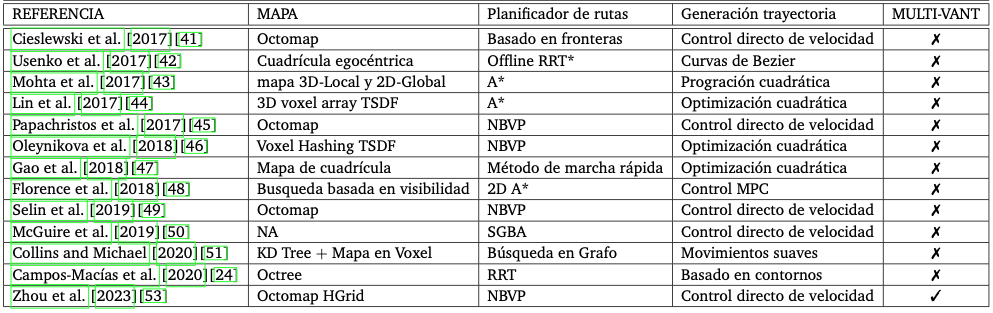
\includegraphics[width=10cm, height=6cm]{estado_del_arte}
%\end{figure}
\end{frame}

\section{Contribuciones o resultados esperados}
\begin{frame}
  \frametitle{Contribuciones o resultados esperados}
  \begin{enumerate}
  \item<1-> Documentación y códigos liberados
    \begin{itemize}
    \item Algoritmo para la exploración multi-VANT
    \item Algoritmo para la planificación de rutas multi-VANT
    \item Protocolo de comunicación y coordinación descentralizados multi-VANT que formaran parte de la arquitectura de software
    \end{itemize}
  \item<2-> Validación de la solución en un simulador
  \item<3-> Tesis impresa
  \end{enumerate}
\end{frame}

\begin{frame}[allowframebreaks,noframenumbering]{Bibliografía}
  \tiny
  \bibliographystyle{abbrvnat}
  \bibliography{test}
\end{frame}

\end{document} 
